\documentclass[runningheads]{llncs}
%
\usepackage[T1]{fontenc}
\usepackage{graphicx}
\usepackage[expansion=false,shrink=10,stretch=10,final]{microtype} % Improved settings
\usepackage{url}  % Add URL package for better URL line breaking
\usepackage[hidelinks,breaklinks,final]{hyperref}
\usepackage{float}
\usepackage{booktabs}


\begin{document}

\raggedbottom
\sloppy

\setlength{\textfloatsep}{10pt plus 2pt minus 4pt}
\setlength{\intextsep}{10pt plus 2pt minus 4pt}

\title{MPDW Project Report --- Phase 3}
\author{David Castro\inst{1,2} \and
Yaroslav Hayduk\inst{1,3} \and
Bruno Baptista\inst{1,4}}
%
% First names are abbreviated in the running head.
% If there are more than two authors, 'et al.' is used.
%
\institute{FCT UNL, Department of Computer Science \and
60973, djc.castro@campus.fct.unl.pt \and
60739, y.hayduk@campus.fct.unl.pt \and
59815, bm.baptista@campus.fct.unl.pt
}
%
\maketitle              % typeset the header of the contribution
%
%\begin{abstract}


%\keywords{First keyword  \and Second keyword \and Another keyword.}
%\end{abstract}
%
%
%
\vspace{2\baselineskip plus 0.5\baselineskip minus 0.5\baselineskip}

\section{Introduction}
This project addresses the challenge of semantic video moment retrieval using transformer-based architectures. The goal is to create a system that can understand user queries and retrieve temporally relevant segments (``video moments'') from long videos.

In phase 1, we focused on understanding and building embedding spaces, indexing video captions, and enabling semantic search using dual encoders and OpenSearch. This involved parsing the \href{https://huggingface.co/datasets/HuggingFaceM4/ActivitiyNet_Captions}{ActivityNet Captions dataset} (used as our base for video content and metadata), selecting key videos and processing their moments, extracting representative keyframes, computing both textual and visual embeddings, and indexing and querying the data using OpenSearch with support for k-nearest-neighbor search.

In Phase 2, we extended this foundation to support cross-modal retrieval and multimodal reasoning. By embedding both captions and keyframes into a shared representation space using CLIP, we enabled text-to-image, image-to-text, and same-modality semantic retrieval. Additionally, we integrated LLaVA, a large vision-language model, to support visual question answering (VQA). In this setup, the system retrieves a relevant video frame for a given visual question and uses LLaVA to generate a natural language response based on the content of that frame.

These additions allow the system to move beyond simple retrieval and support more complex, open-ended interaction with video content through both cross-modal search and generative question answering.

To gain deeper insight into model behavior, we also explored CLIP interpretability by visualizing similarity scores and attention heatmaps between captions and video frames.


\vspace{2\baselineskip plus 0.5\baselineskip minus 0.5\baselineskip} % space sections out

\pagebreak

\section{System Architecture}
Our Phase 2 system forms a five-stage pipeline that converts raw ActivityNet videos into an indexable,
query-able, and interpretable LVLM service.

\begin{enumerate}
  \item \textbf{Pre-processing}  
        \begin{itemize}
        \item Trim videos to annotated moments and extract key-frames.
        \item Merge timestamped captions from \texttt{val\_1.json} and \texttt{val\_2.json}.
        \end{itemize}
  \item \textbf{Multimodal Embedding Generation}  
        \begin{itemize}
        \item \emph{Sentence-BERT MPNet} $\!\to$ 768-d \texttt{caption\_vec} (semantic text search).  
        \item \emph{CLIP ViT-B/32 -- text encoder} $\!\to$ 512-d \texttt{visual\_caption\_vec}.  
        \item \emph{CLIP ViT-B/32 -- image encoder} $\!\to$512-d \texttt{keyframe\_vec}.
        \end{itemize}
  \item \textbf{Indexing (OpenSearch)}  
        Three \texttt{knn\_vector} fields, HNSW (\texttt{M}=16, \texttt{ef}=256), plus metadata (timestamps, resolution).
  \item \textbf{Cross-modal Retrieval API}  
        \texttt{search(query, modality)} dispatches to one of  
        \textit{text$\!\to$image}, \textit{image$\!\to$text}, \textit{image$\!\to$image} and returns top-\(k\) ranked hits.
  \item \textbf{Retrieval-Augmented VQA}  
        The best key-frame is fed, together with the user question, to \emph{LLaVA-Phi-3}.  
        Answers and CLIP similarities are cached and logged.
  \item \textbf{Interpretability Module}  
        Generates (i) temporal similarity curves, (ii) Grad-CAM heat-maps for 10 frames, and (iii) a caption × frame
        contrastive matrix.
\end{enumerate}
\pagebreak[3]

\subsection{Embedding Representations and Index Schema}
We moved from a \emph{dual} to a \textbf{tri-encoder} design so that the text and image
branches share the same CLIP space.  
Three independent vector fields are written to OpenSearch (Table~\ref{tab:fields}).

\begin{itemize}
  \item \textbf{Sentence-BERT (MPNet)}  
        Captions $\rightarrow$ 768-d \texttt{caption\_vec}.  
        Used for classic semantic \emph{text$\!\to$text} retrieval baselines.
  \item \textbf{CLIP ViT-B/32 — text encoder}  
        Captions $\rightarrow$ 512-d \texttt{visual\_caption\_vec}.  
        Aligns captions with images and enables \emph{text$\!\to$image} queries.
  \item \textbf{CLIP ViT-B/32 — image encoder}  
        Key-frames $\rightarrow$ 512-d \texttt{keyframe\_vec}.  
        Supports \emph{image$\!\to$image} and \emph{image$\!\to$text}.
\end{itemize}

\begin{table}[h]
\centering
\begin{tabular}{lcc}
\toprule
Field & Model & Dim. \\ \midrule
\texttt{caption\_vec} & SBERT MPNet & 768 \\
\texttt{visual\_caption\_vec} & CLIP (text) & 512 \\
\texttt{keyframe\_vec} & CLIP (image) & 512 \\ \bottomrule
\end{tabular}\label{tab:fields}
\end{table}

\begin{sloppypar}
\textbf{Document granularity.}  
One index document corresponds to a \emph{(key-frame, caption)} pair.  
A key-frame that overlaps two temporal moments is therefore duplicated, each time
with the relevant caption and its own ID.  
Metadata stored alongside the vectors now includes:  
\texttt{video\_id}, \texttt{start\_timestamp}, \texttt{end\_timestamp},
\texttt{duration}, \texttt{resolution}, and the local \texttt{keyframe\_path}.
All vectors are $\ell_2$-normalised before insertion so cosine similarity reduces
to the inner-product HNSW metric configured in OpenSearch.
\end{sloppypar}


\paragraph{Contextual embeddings:}For visualizing contextual embeddings, we utilized the caption of one of our videos: 
``A man is in a skateboard track, then he throws a bowling ball that goes around and hits the pins''. 
The resulting graphs of the layers zero to eleven can be seen in Fig.~\ref{hidden_layers}.

\vspace{2\baselineskip plus 0.5\baselineskip minus 0.5\baselineskip} 


\begin{figure}[H]
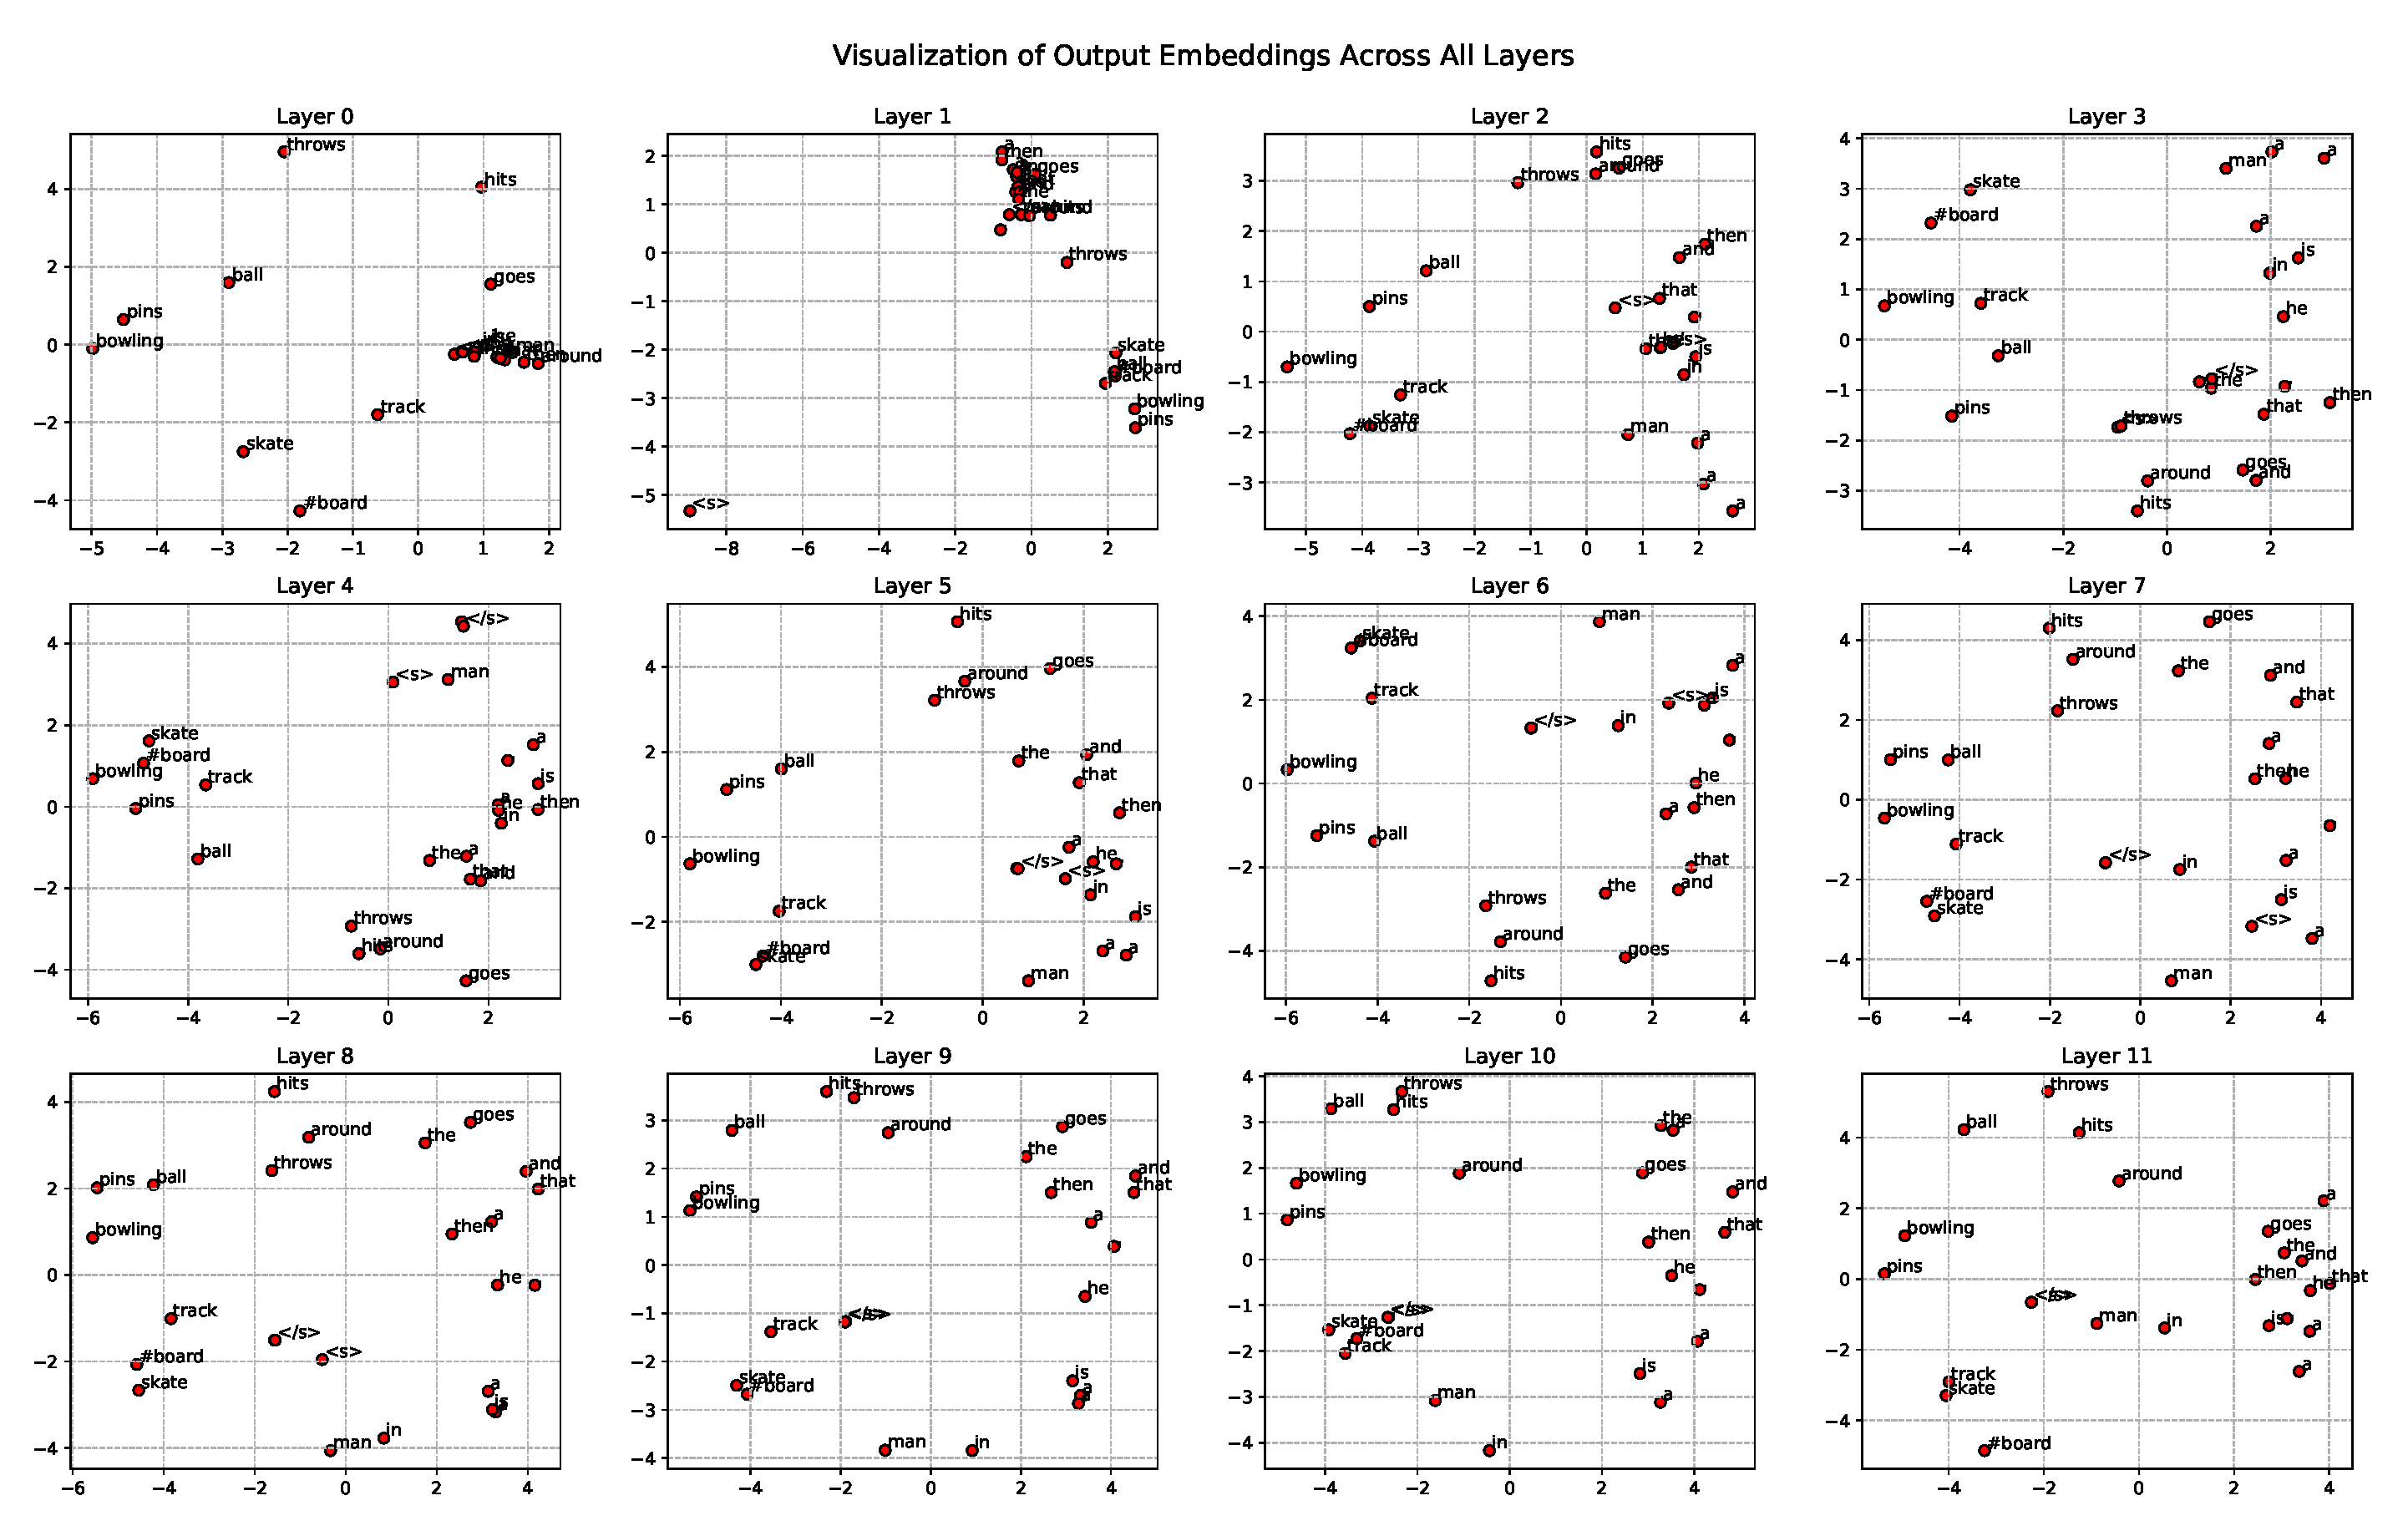
\includegraphics[width=0.95\textwidth]{../figures/hidden_layers.eps}
\caption{Contextual embeddings}\label{hidden_layers}
\end{figure}

\vspace{2\baselineskip plus 0.5\baselineskip minus 0.5\baselineskip} 

Surprisingly, in the first layer, the embeddings are very similar to their values in the eleventh layer, but this outcome is merely coincidental, while in the second layer we get something that would be more expected, that is, most embeddings are fairly close together with seemingly no relation or logic. With the progression of the layers, we can see the embeddings disperse and form sensible groups. Namely, we can see the terms ``bowling'' and ``pins'' very close together and far from most other words. This makes sense given how specific and relatively rare those words are. The same can be observed for skate, track and board --- the suffix of skateboard, hence the proximity. Lastly, the most obvious cluster, on the right: the most common english words. Words such as ``a'', ``the'', ``that'' and ``and'' which, due to the frequent and indiscriminate use that is given to them, hold very little semantic value and weight in the meaning of sentences.


\paragraph{Positional embeddings:}By repeating the previous exercise with a sentence of the same word repeated 20 times instead, what we get is the positional embeddings of our sentence (see Fig.~\ref{pos_embeds}). The result is a phenomenon that can be explained by the gradual decrease of positional importance throughout the sentence. Stated in simpler terms, the farther a token is from the first word, the smaller the importance of its position. The first word is the one we can see down at the bottom, the farthest from all the others, as its position has the highest relevance. As we move forth in the sentence, the position relevance gradually decreases and we get increasingly similar embeddings. Due to this, we see the converging effect that results in the cluster of points we see at the top, with all the embeddings of the last words close together.

\vspace{3\baselineskip plus 0.5\baselineskip minus 0.5\baselineskip} 

\begin{figure}[!htb]
  \centering
  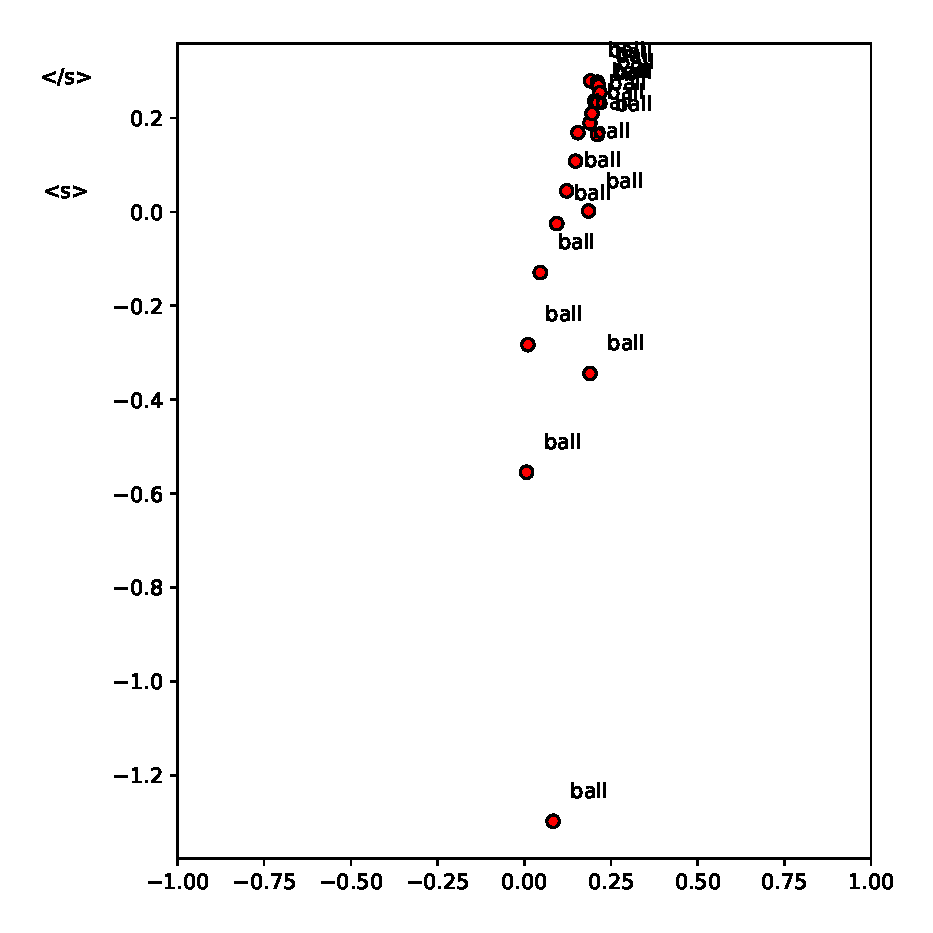
\includegraphics[width=.5\textwidth, clip=true, trim = 15mm 0mm 0mm 0mm]{../figures/pos_embeds.eps}
  \caption{Positional embeddings}\label{pos_embeds}\label{img:positional_embeddings}
\end{figure}

\clearpage


\subsection{Large Vision and Language Models}
While Phase 2 delves deeper into large vision and language models, in Phase 1 we already used pretrained transformers:

\begin{itemize}
    \item \textbf{MPNet (All-MPNet-Base-V2)} for generating context-aware text embeddings.
    \item \textbf{CLIP (ViT-B/32)} to embed keyframes into a multimodal representation space.
\end{itemize}

In Phase 2, we extended the use of CLIP to achieve full \textbf{cross-modal retrieval} functionality by embedding both keyframes and captions using CLIP’s respective image and text encoders. This allows us to represent both modalities in the same embedding space, enabling:

\begin{itemize}
    \item \textbf{Text-to-image retrieval}, where a natural language query retrieves relevant keyframes.

    \item \textbf{Image-to-text retrieval}, where a visual frame can retrieve semantically aligned captions.

    \item \textbf{Image-to-image} and \textbf{text-to-text retrieval}, leveraging the shared embedding space for similarity search across same-modality inputs.
\end{itemize}

All CLIP embeddings, whether from keyframes or captions, were indexed in OpenSearch, allowing for real-time similarity search.

We also integrated \textbf{LLaVA (Large Language and Vision Assistant)} for visual question answering (VQA). LLaVA combines CLIP’s visual encoder with a language model fine-tuned for multimodal reasoning.

In our system, we used retrieval-augmented VQA:

\begin{enumerate}
    \item A visual question is submitted.

    \item The embedding for the question is computed using CLIP's text encoder.

    \item A k-NN search is performed to retrieve the most relevant keyframe based on semantic similarity in the shared embedding space.

    \item Both the retrieved frame and the question are passed to LLaVA.

    \item LLaVA returns a grounded, natural language answer to the question based on the content of the frame.
\end{enumerate}

Below are a couple of examples of the usage of LLaVa:

\textbf{Question 1}

Question: \textit{"What is the man doing at the skatepark?"}

Retrieved Frame: Fig.~\ref{retrived-frame-1}

Generated answer: The image shows a group of people, including a young person and others, gathered around a skateboard ramp in an outdoor skate park. One boy with a skateboard is positioned on top of a half-pipe, seemingly preparing to ride down it or possibly just finished his run. The man standing by the side of the ramp could be observing, watching the skateboarder, providing assistance, or waiting for his turn. There are also several chairs visible in the area, which might provide a place for spectators to sit and watch the activities at the skate park.

\textbf{Question 2}

Question: \textit{"What color are the boxing gloves?"}

Retrieved Frame: Fig.~\ref{retrived-frame-2}

Generated answer: The boxing gloves in the image are red.

\textbf{Question 3}

Question: \textit{"Where is the man playing bowling?"}

Retrieved Frame: Fig.~\ref{retrived-frame-3}

Generated answer: Inside a building, specifically in an indoor alley.


\begin{figure}[!htb]
  \centering
  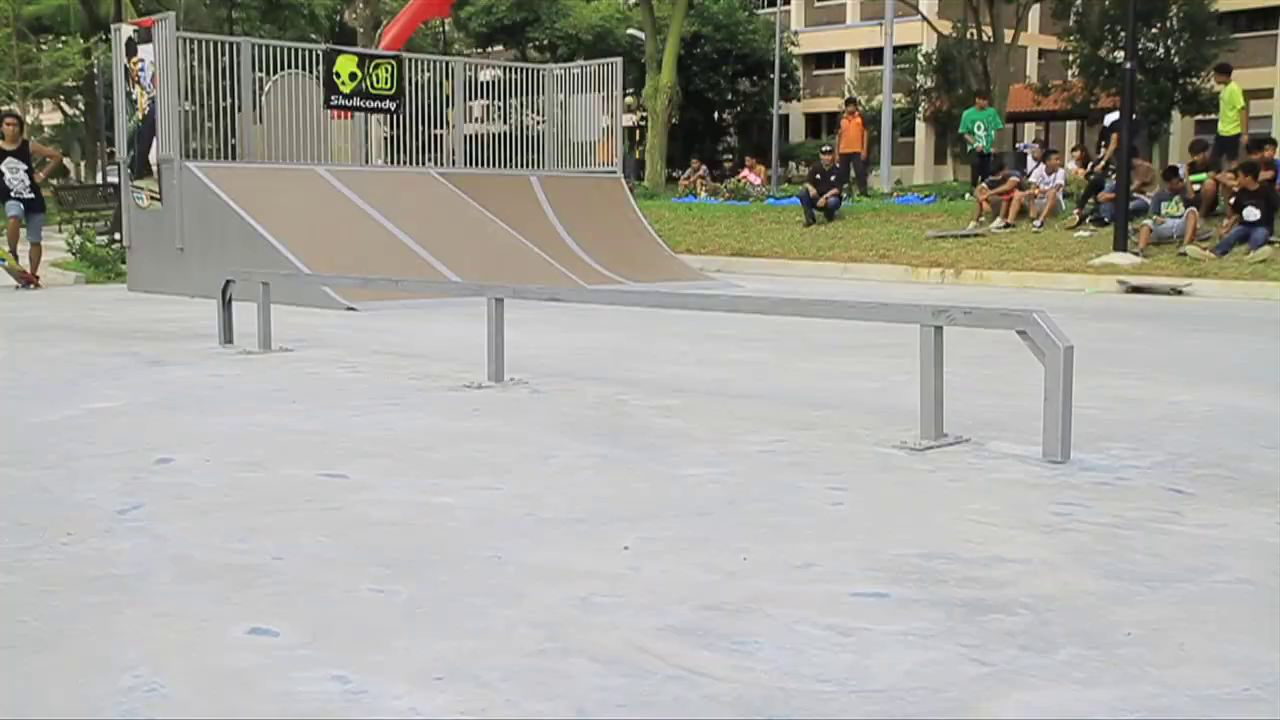
\includegraphics[width=0.9\textwidth, clip=true]{../figures/example_1.png}
  \caption{Retrieved frame for question "What is the man doing at the skatepark?"}\label{retrived-frame-1}
\end{figure}

\begin{figure}[!htb]
  \centering
  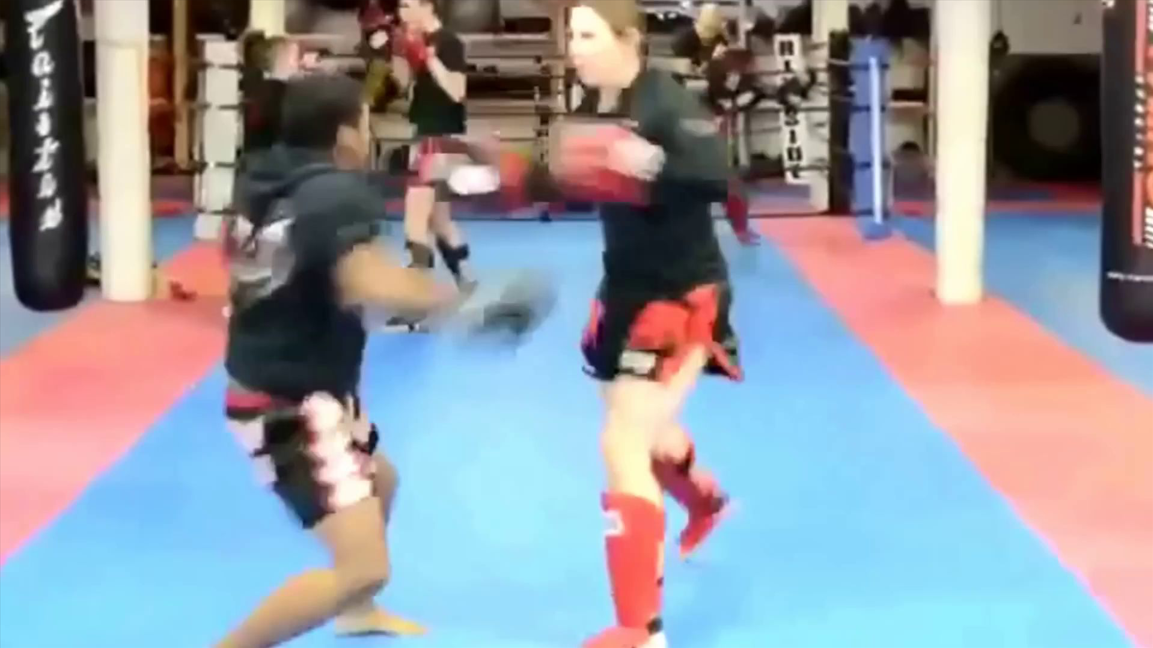
\includegraphics[width=0.9\textwidth, clip=true]{../figures/example_2.png}
  \caption{Retrieved frame for question "What color are the boxing gloves?"}\label{retrived-frame-2}
\end{figure}

\begin{figure}[!htb]
  \centering
  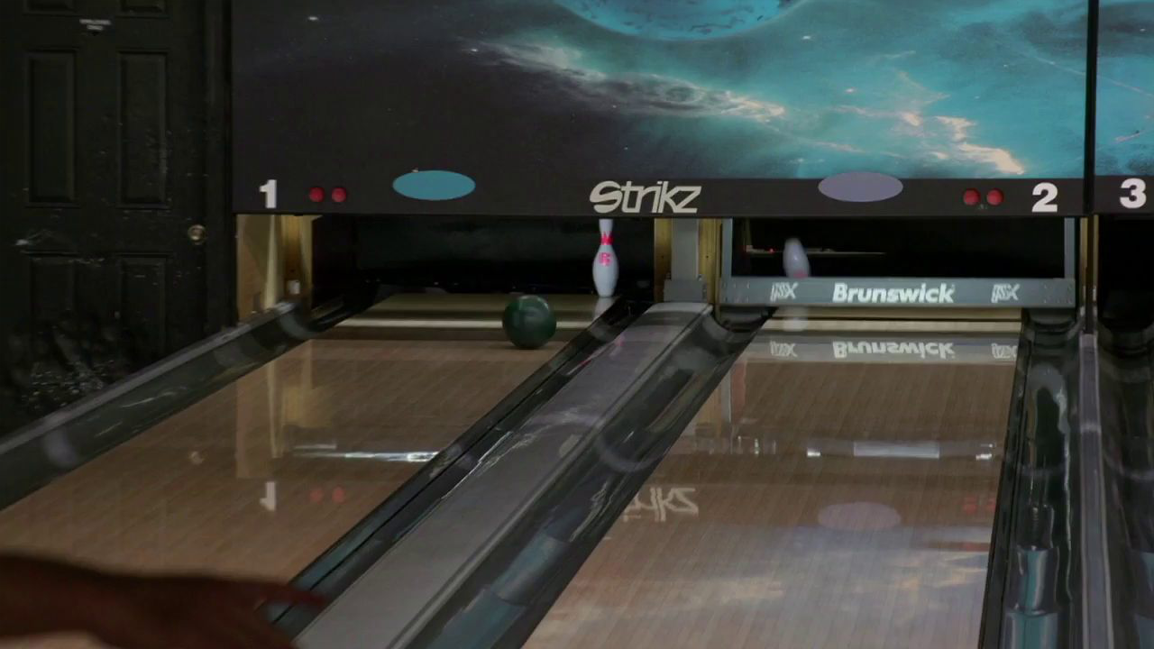
\includegraphics[width=0.9\textwidth, clip=true]{../figures/example_3.png}
  \caption{Retrieved frame for question "Where is the man playing bowling?"}\label{retrived-frame-3}
\end{figure}


\subsection{Attention}


\paragraph{Self-attention for Cross-Encoder:} To analyze the model's self-attention mechanism we generated every head's self-attention for the input ``where is the man? A man is in a skateboard track, then he throws a bowling ball that goes around and hits the pins''. When looking at the different heads there are multiple patterns we can identify, giving us an intuition of their purpose. A lot of them also simply pay a general, overall attention to the whole sentence. If we look at figure~\ref{self_att_heads}, head 2 looks at every token relatively the same, with a special interest in itself, given the distinctive diagonal. This phenomenon can be seen even more clearly in head 7. Head 3 shows us a very clear diagonal pattern, where each token pays higher attention to itself and the around 3 to 6 right next to it, with virtually no attention to all the others; this could be loosely interpreted as: this head solely pays attention to the current token and the few right next to it. Similar effects can be seen in other heads, such as head 6, 9 and 11. Head 6 seems to be paying most of its attention to the couple of tokens right before and right after the current token. Head 9 attends pretty much only to the two tokens right behind the current token. While finally, head 11, pays attention almost exclusively to the token immediately after.

\vspace{2\baselineskip plus 0.5\baselineskip minus 0.5\baselineskip} % Add space between sections
% \clearpage

\paragraph{Self-Attention for Dual-Encoder:} 
In the dual-encoder architecture, the query and document are processed independently, which results in separate self-attention mechanisms for each. To analyze this, we visualized the attention heads for both the query sequence \textit{``Where is the man?''} and the document \textit{``A man is in a skateboard track, then he throws a bowling ball that goes around and hits the pins''}, as shown in Figures~\ref{self_att_document} and~\ref{self_att_query}.

For the query, attention patterns are more localized and interpretable due to its short length. Many heads show weak diagonals, indicating that each token attends mostly to those ahead of it.
In contrast, the document's self-attention shows more diverse behavior. Several heads focus attention across broader spans of the input, capturing syntactic structures or semantic relations within the sentence. For instance, tokens such as \textit{``skate''} or \textit{``hits''} often receive and distribute attention across related nouns like \textit{``board''} or \textit{``pins''}, suggesting an awareness of action-object relationships. Other heads demonstrate local attention, where each token mainly attends to subsequent neighbors.

Unlike the cross-encoder, the dual-encoder architecture does not allow for query-document token interaction within the attention layers. Instead, it relies on the resulting embeddings of the entire sequences to compute similarity. We can clearly see from our results how similar their embeddings are, which greatly enhances that operation's precision.

\vspace{2\baselineskip plus 0.5\baselineskip minus 0.5\baselineskip} % Add space between sections

\begin{figure}[!htb]
  \centering
  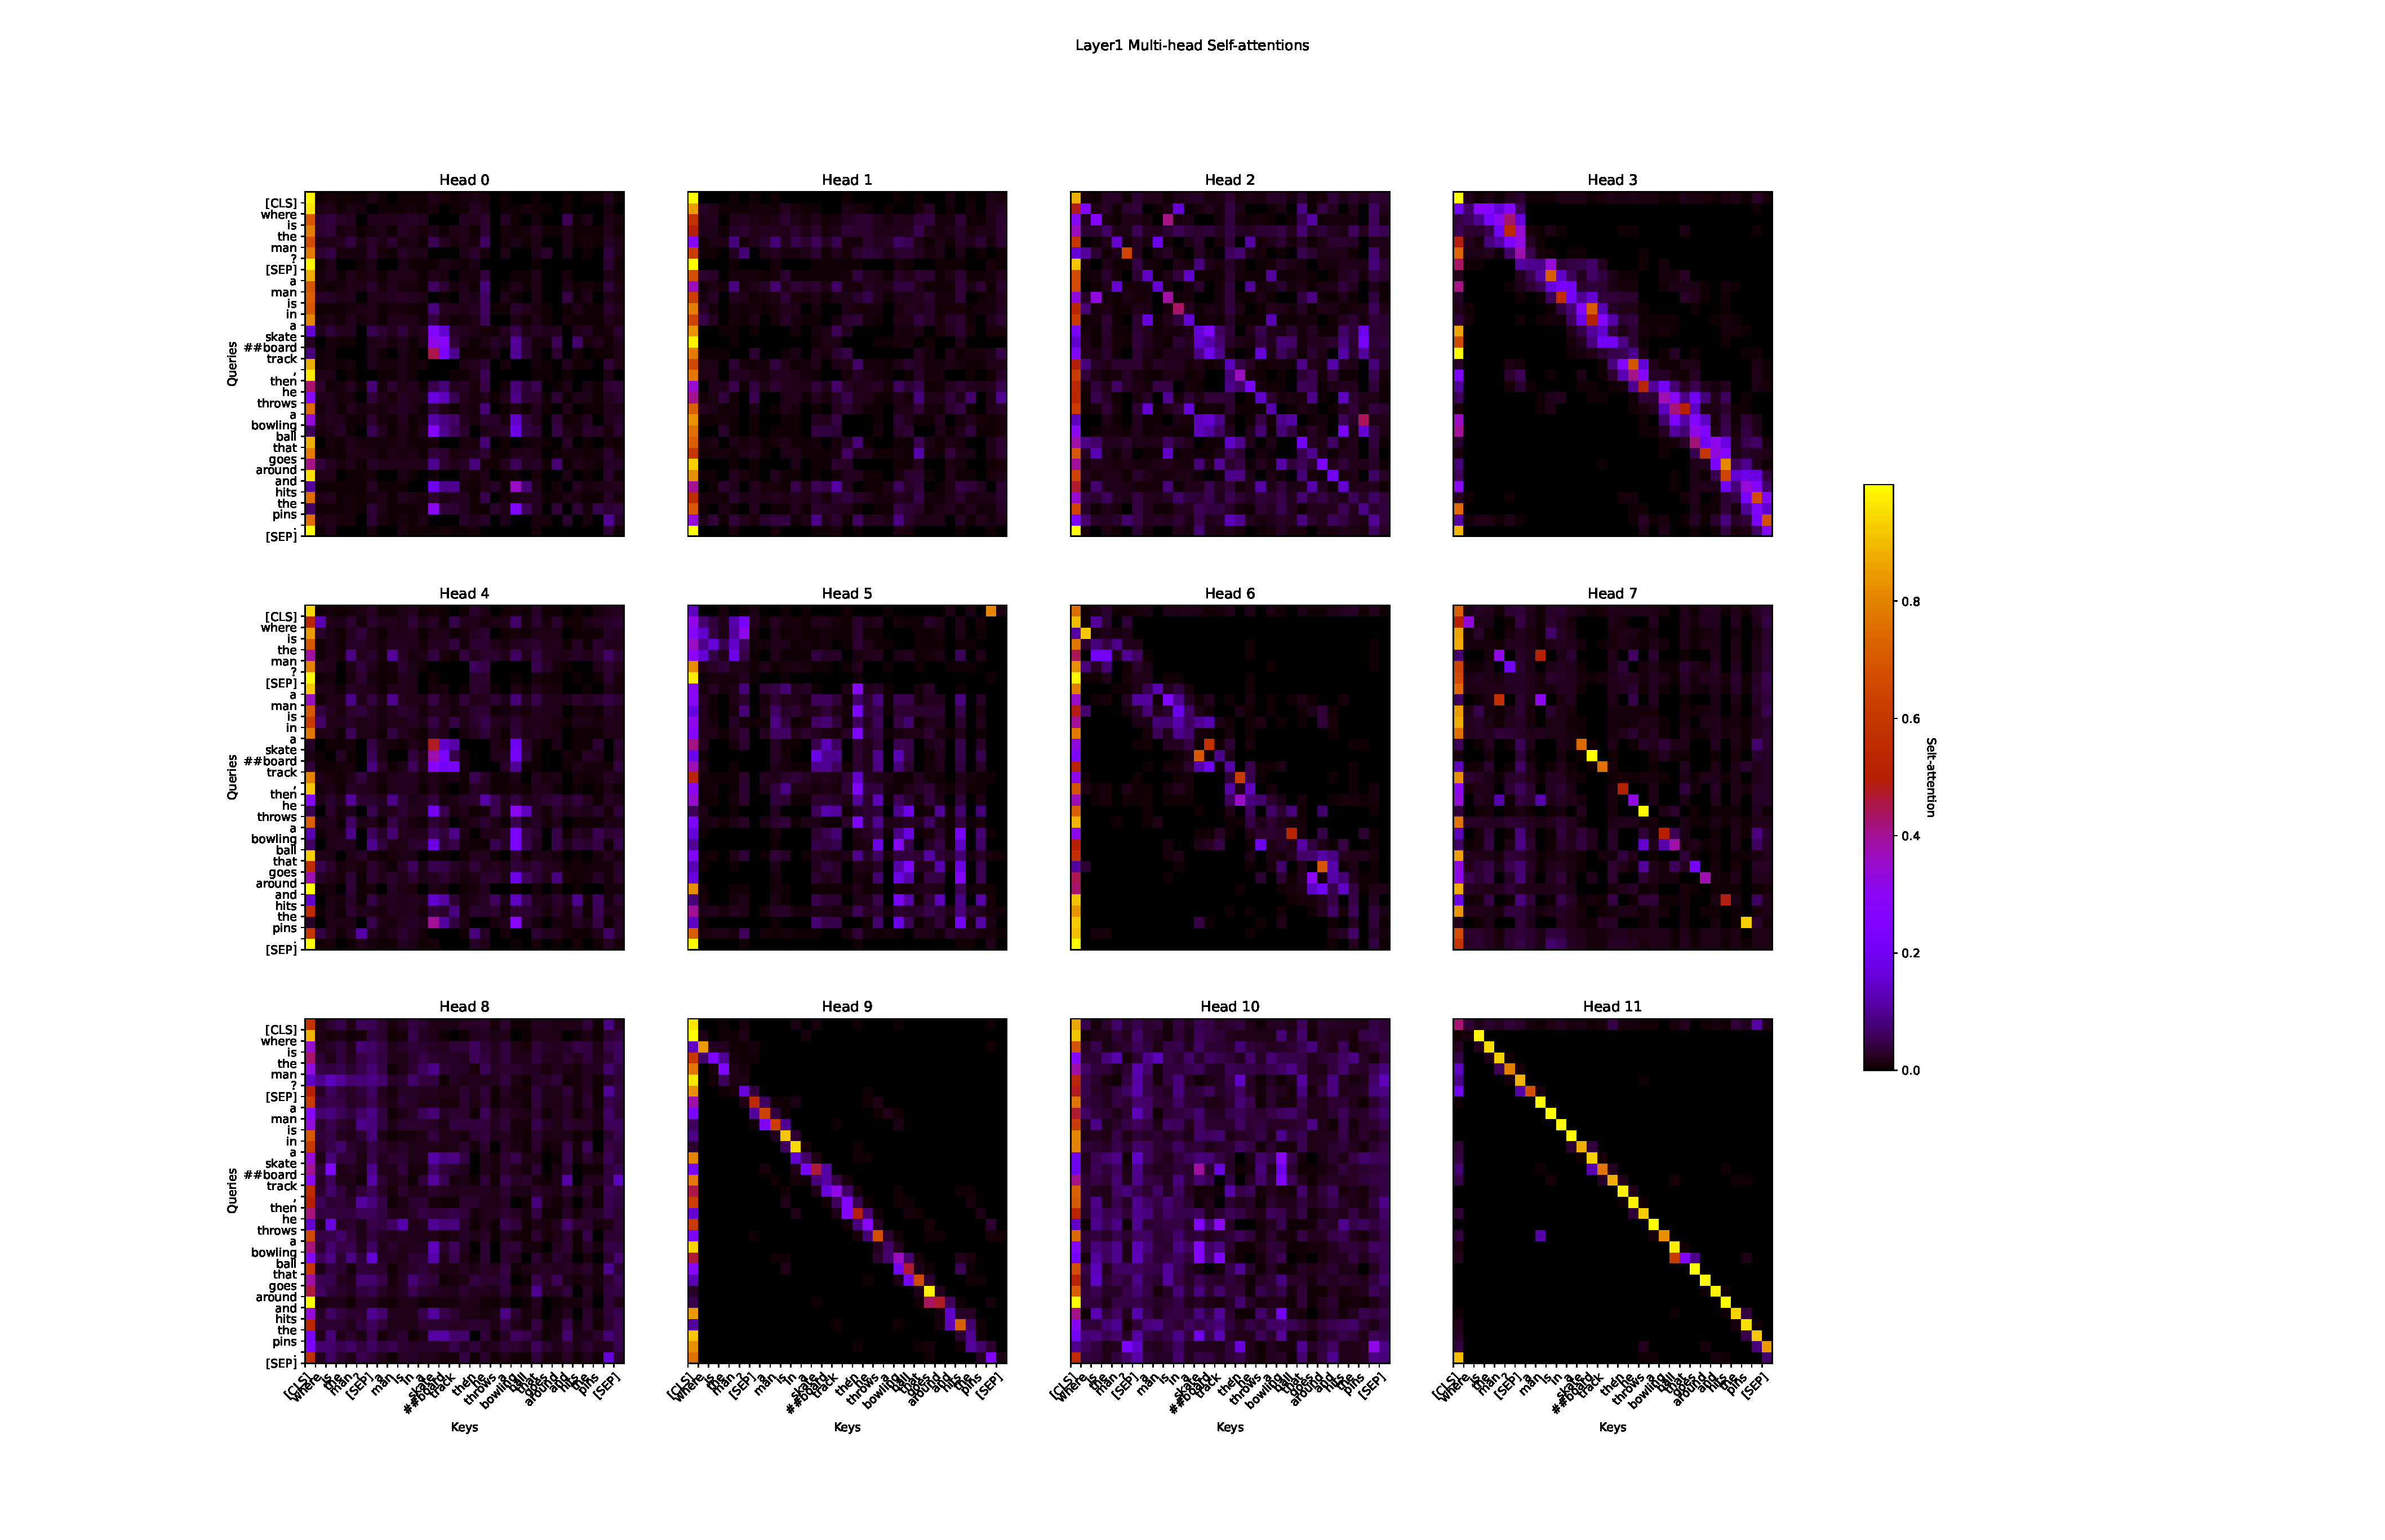
\includegraphics[width=0.95\textwidth, clip=true, trim = 70mm 25mm 130mm 45mm]{../figures/self_att_heads.eps}
  \caption{Self-attention}\label{self_att_heads}\label{img:self_attention}
\end{figure}

\clearpage

\begin{figure}[!htb]
  \centering
  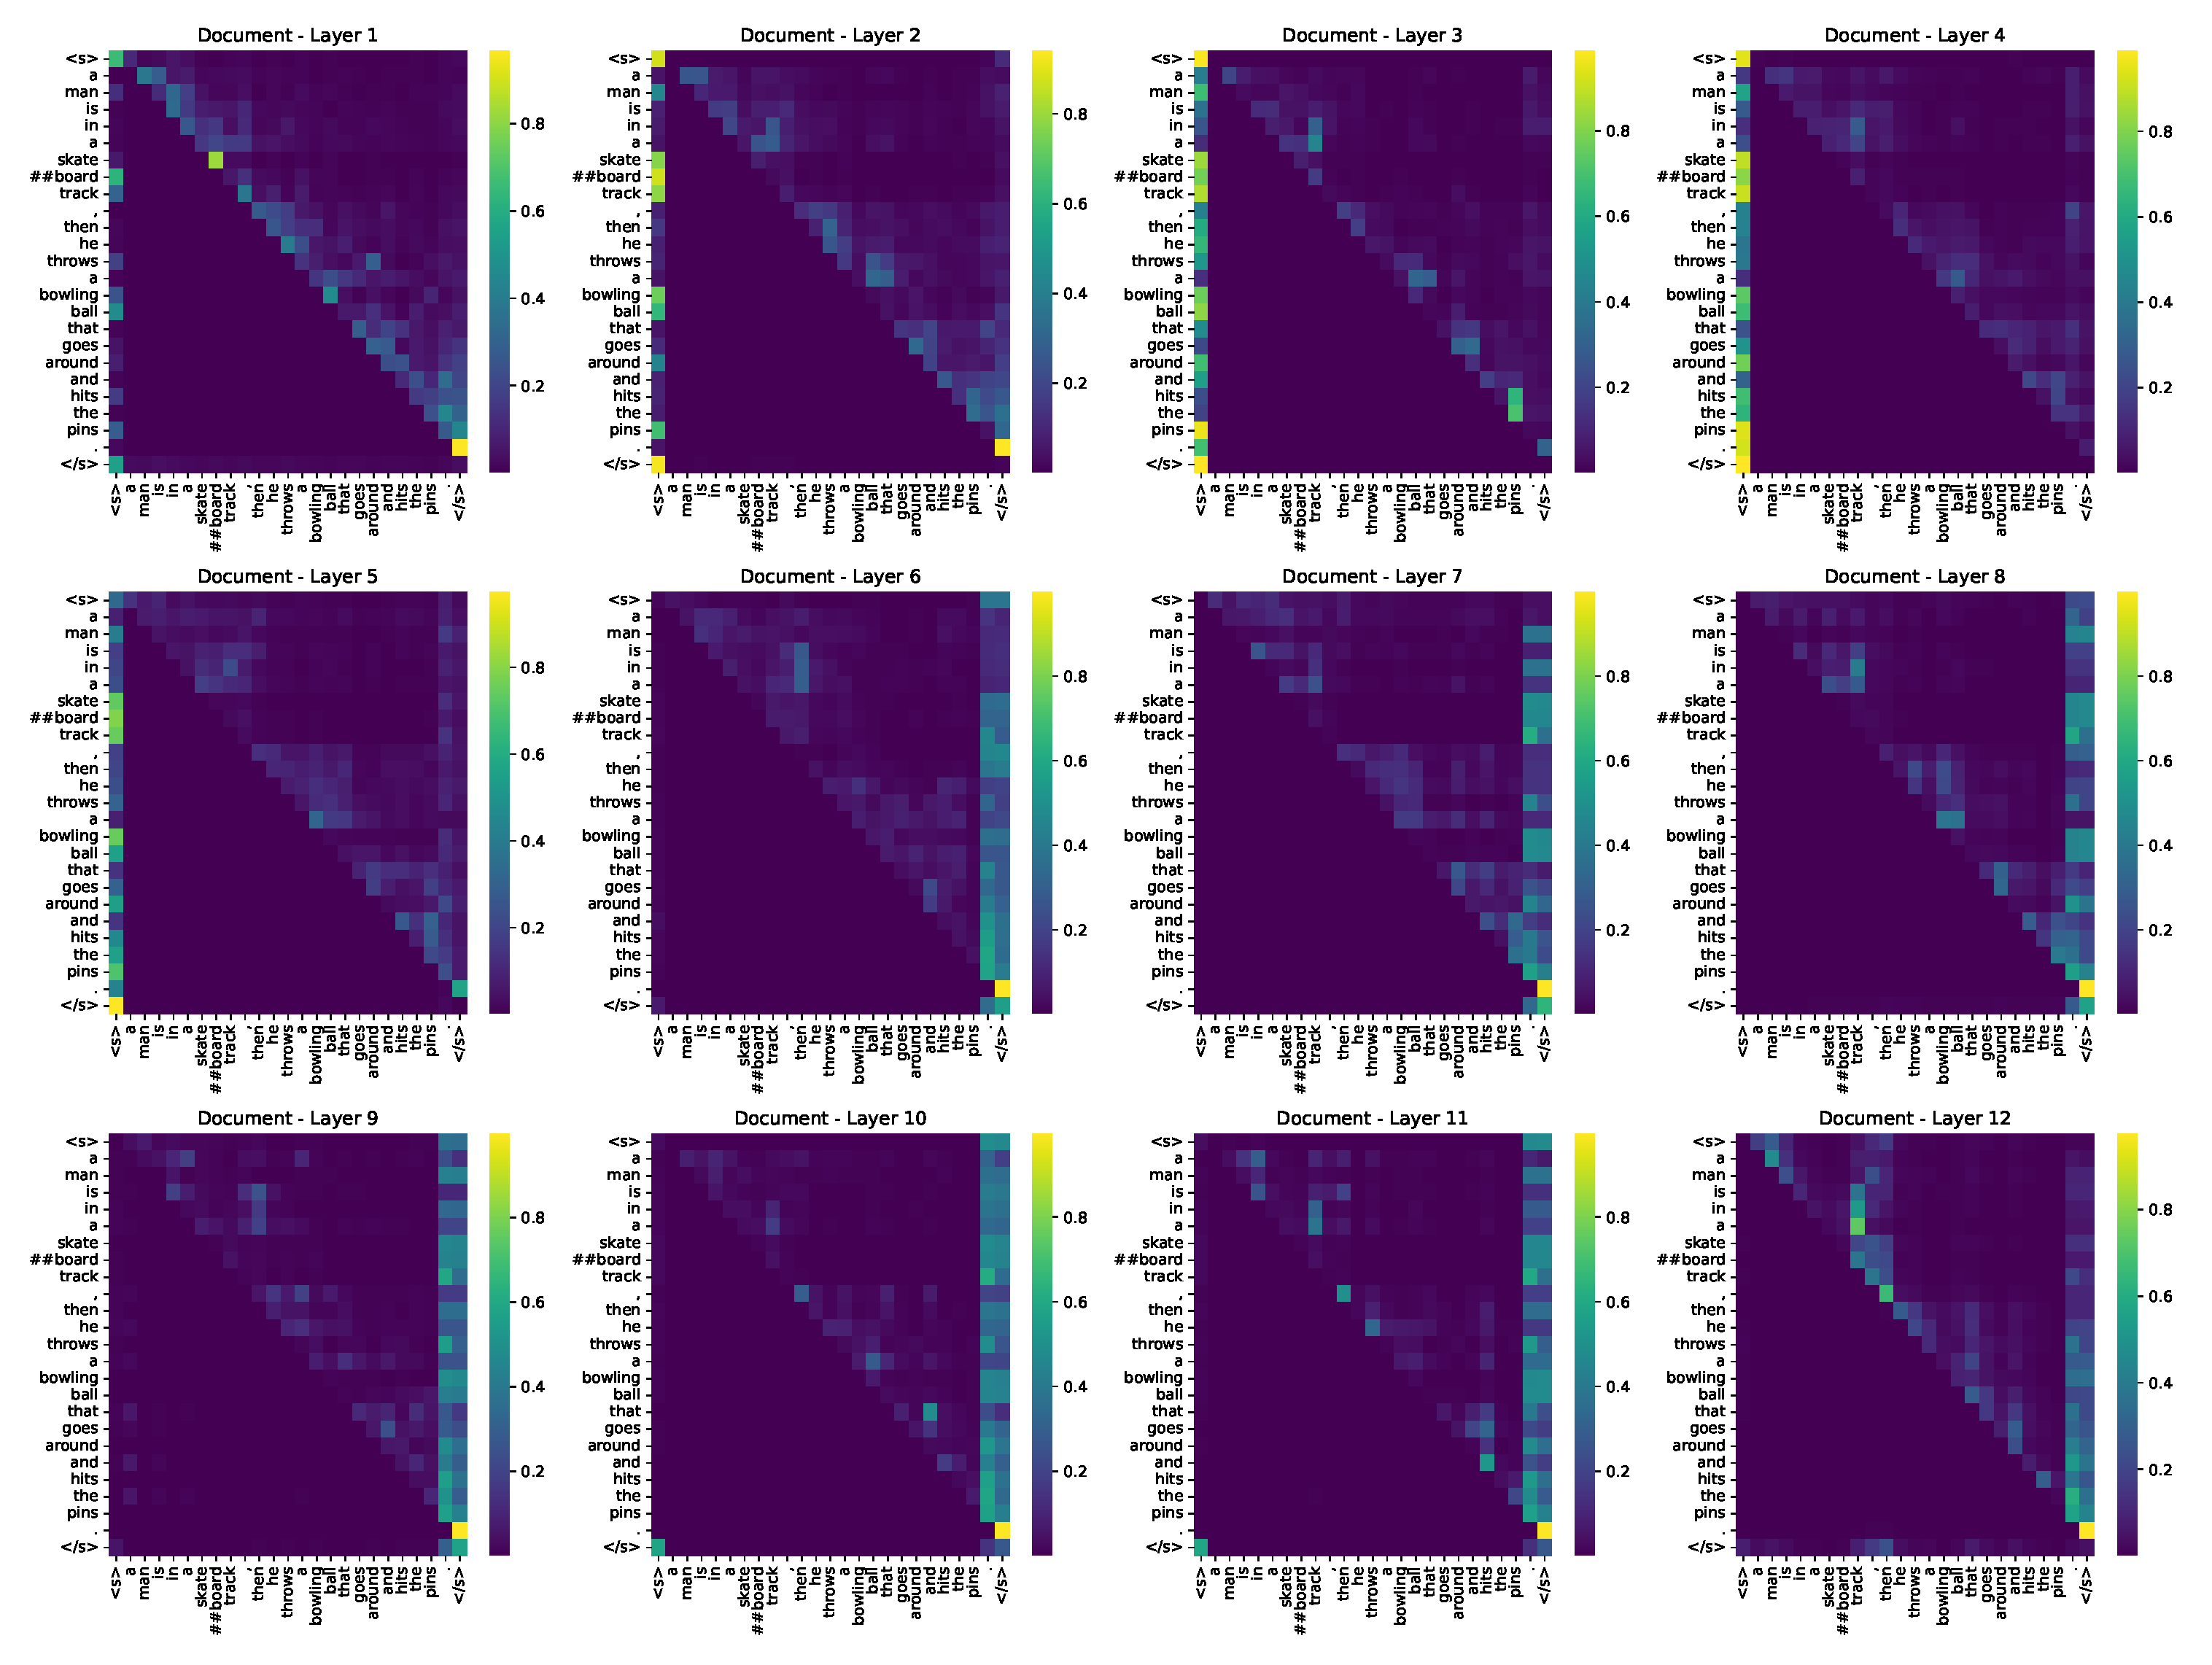
\includegraphics[width=0.90\textwidth, clip=true]{../figures/attention_layers_document.eps}
  \caption{Self-attention document}\label{self_att_document}\label{img:self_attention_document}
\end{figure}


\begin{figure}[!htb]
  \centering
  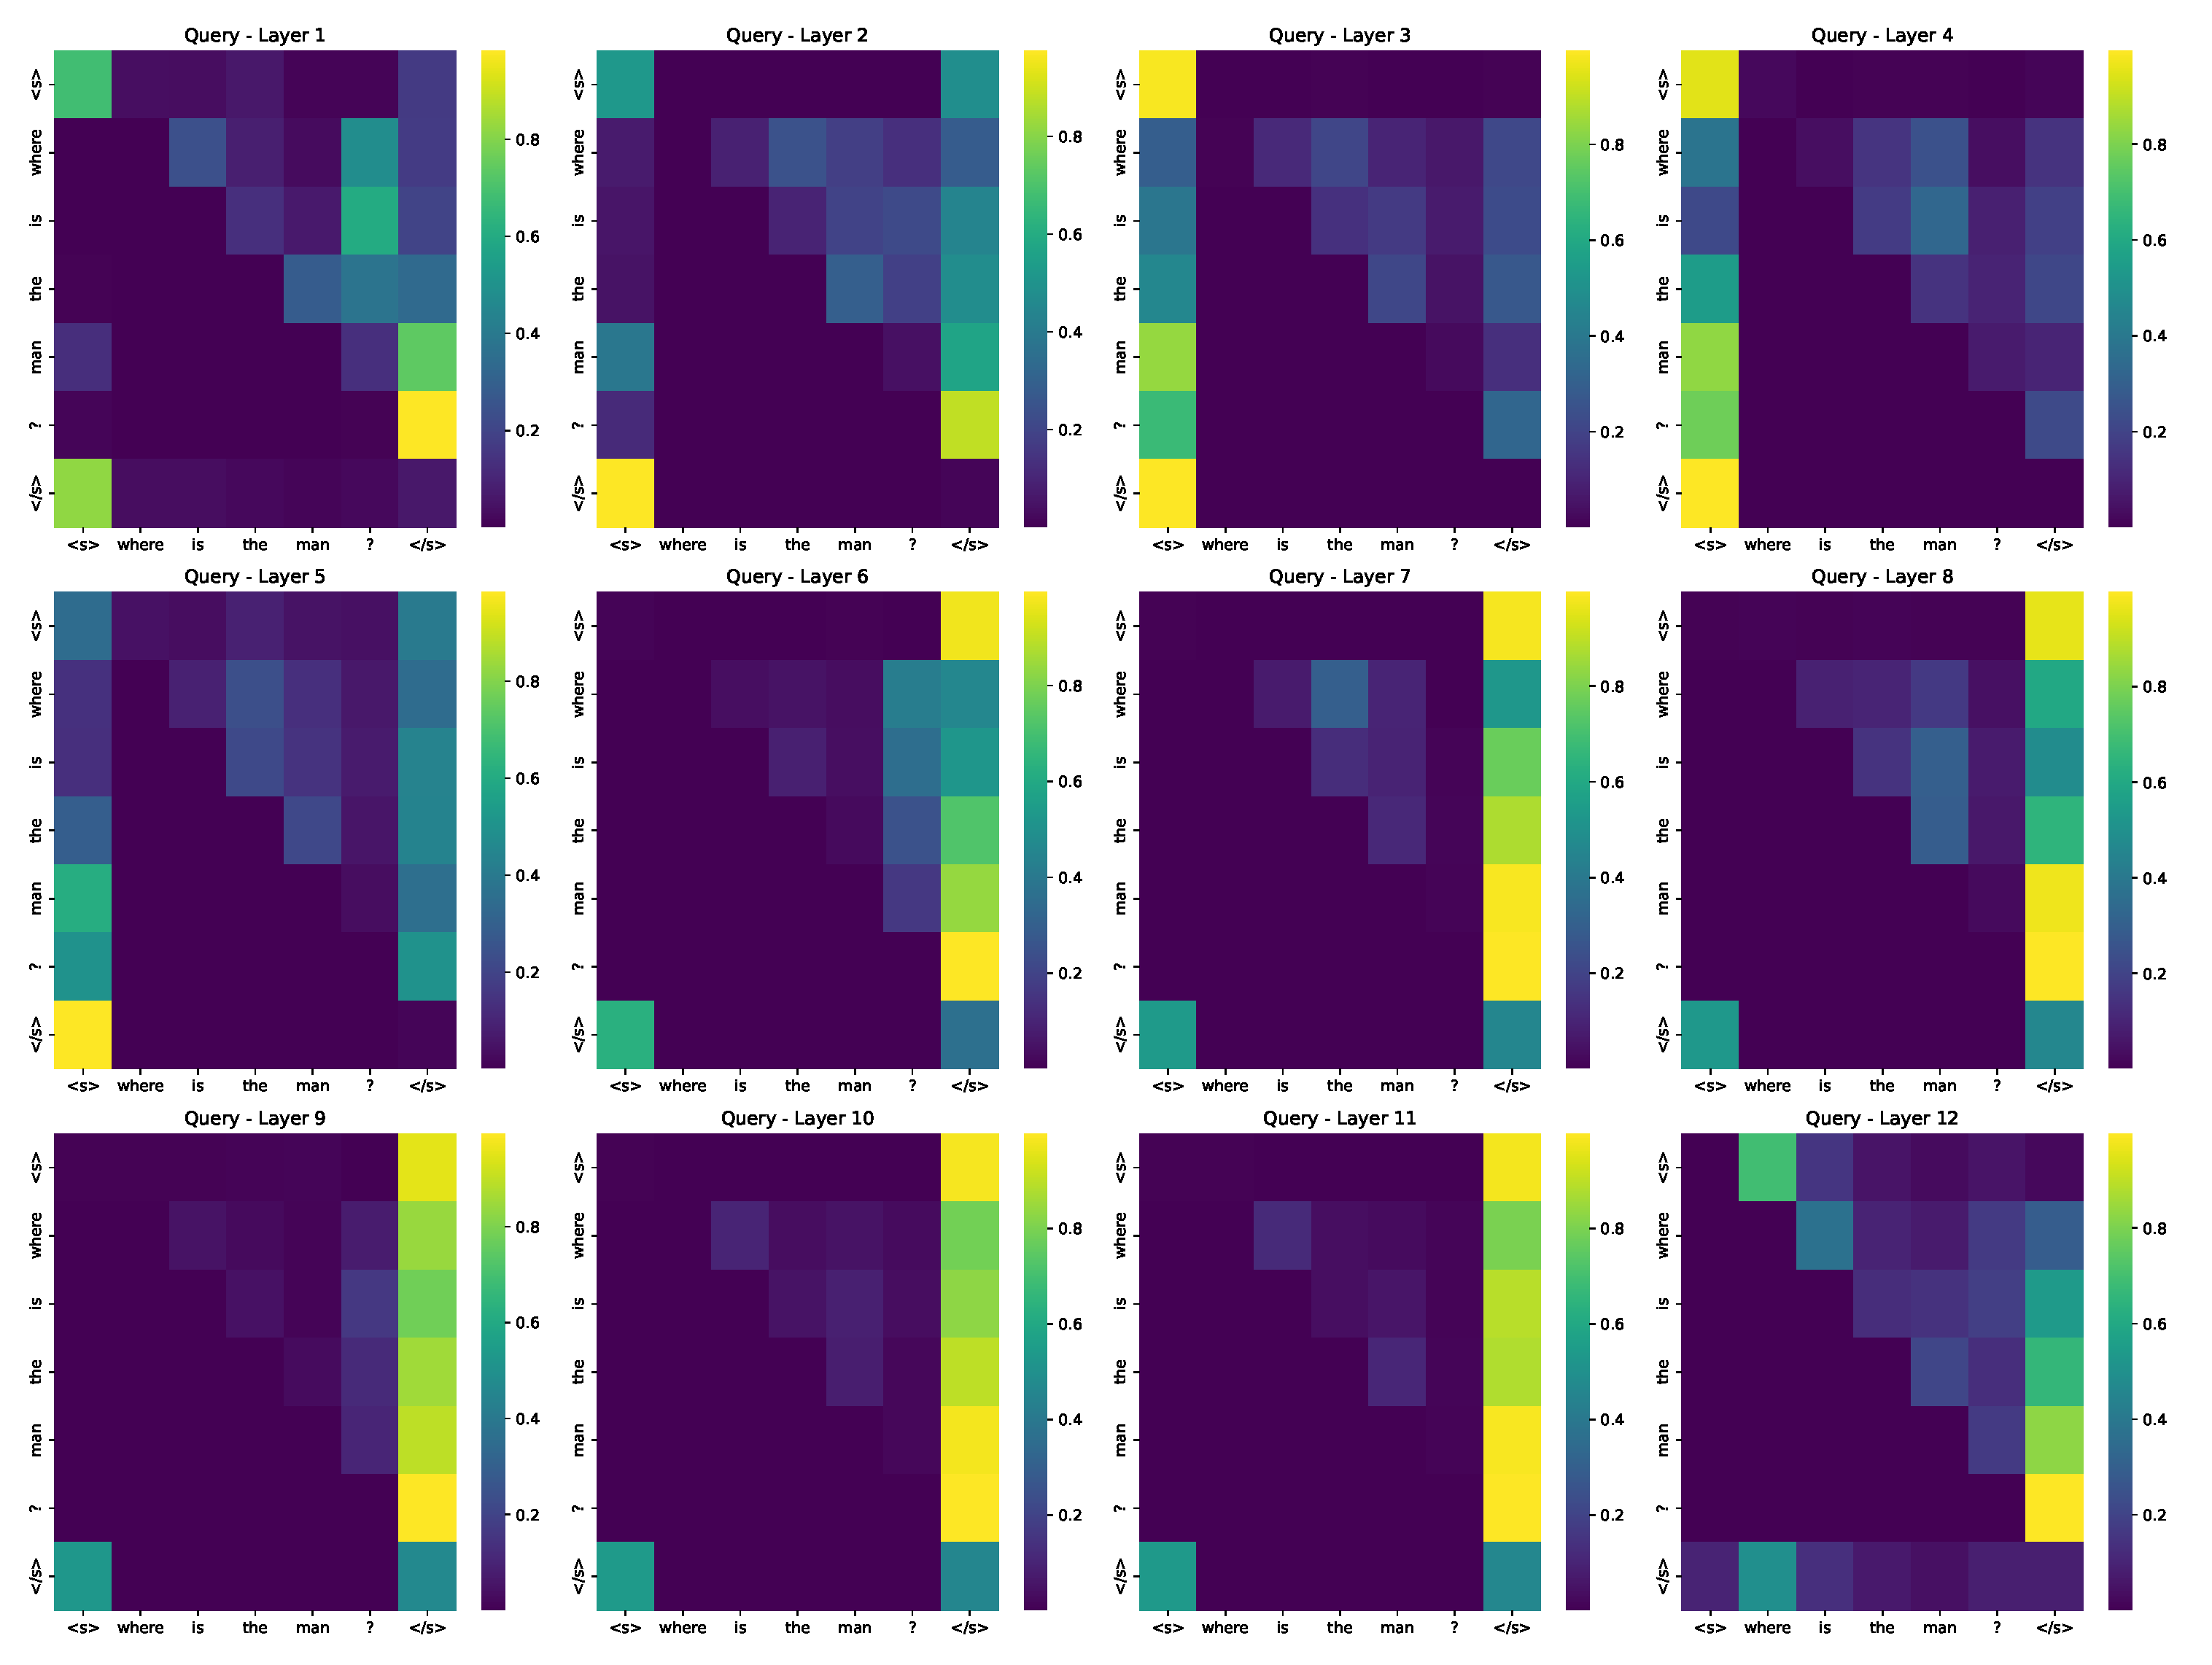
\includegraphics[width=0.9\textwidth, clip=true]{../figures/attention_layers_query.eps}
  \caption{Self-attention query}\label{self_att_query}\label{img:self_attention_query}
\end{figure}

\clearpage

\vspace{2\baselineskip plus 0.5\baselineskip minus 0.5\baselineskip} % space sections out

\subsection{CLIP Interpretability}

In this section, we interpret the embeddings generated by our CLIP model for both images and text, and the relation they display with each other, as well as analyze its attention mechanism and a representation of it.

\subsubsection{Language-Vision temporal similarity}
To analyze the temporal similarity between a caption and a video, we selected a video along with all its frames, chose a caption, and computed the similarity between its CLIP embedding and the embeddings of each frame in the video. For our particular example the caption was '\textit{Two men interview each other on brown chairs}', belonging to a segment of a video by \textit{Dude Perfect}, where they perform multiple bowling ball shenanigans, with the results shown in Fig.\ref{cap-frame-sim-score-1}. In order to obtain a smoother graph,, we averaged each point with the one immediately before and immediately after. In this figure, we are able to see the sections where the similarity score is highest, and where is lowest (apart from the beginning and ending), along with a small thumbnail of the frame for ease of analysis. As we can clearly observe, the similarity score is fairly low throughout the video, as most of it features said bowling shenanigans; but when it cuts to the interview section, the one that exactly corresponds to the two men interviewing each other, it spikes up, resulting in the effect we see. Worth noting is the other big spike we see before that, corresponding also to two men interviewing each other, although not on brown chairs. The lowest point we see features neither men interviewing each other nor brown chairs, accounting for the low similarity score. The particular spike down, in comparison to other moments, can be explained by the fact that throughout the video, in short segments are featured the \textit{dudes} from \textit{dude perfect} briefly speaking to each other - possibly being interpreted as some form of \textit{two men interviewing each other} -, while this part, around frame 55, is mostly just bowling a bowling ball trickshot.

\begin{figure}[!htb]
  \centering
  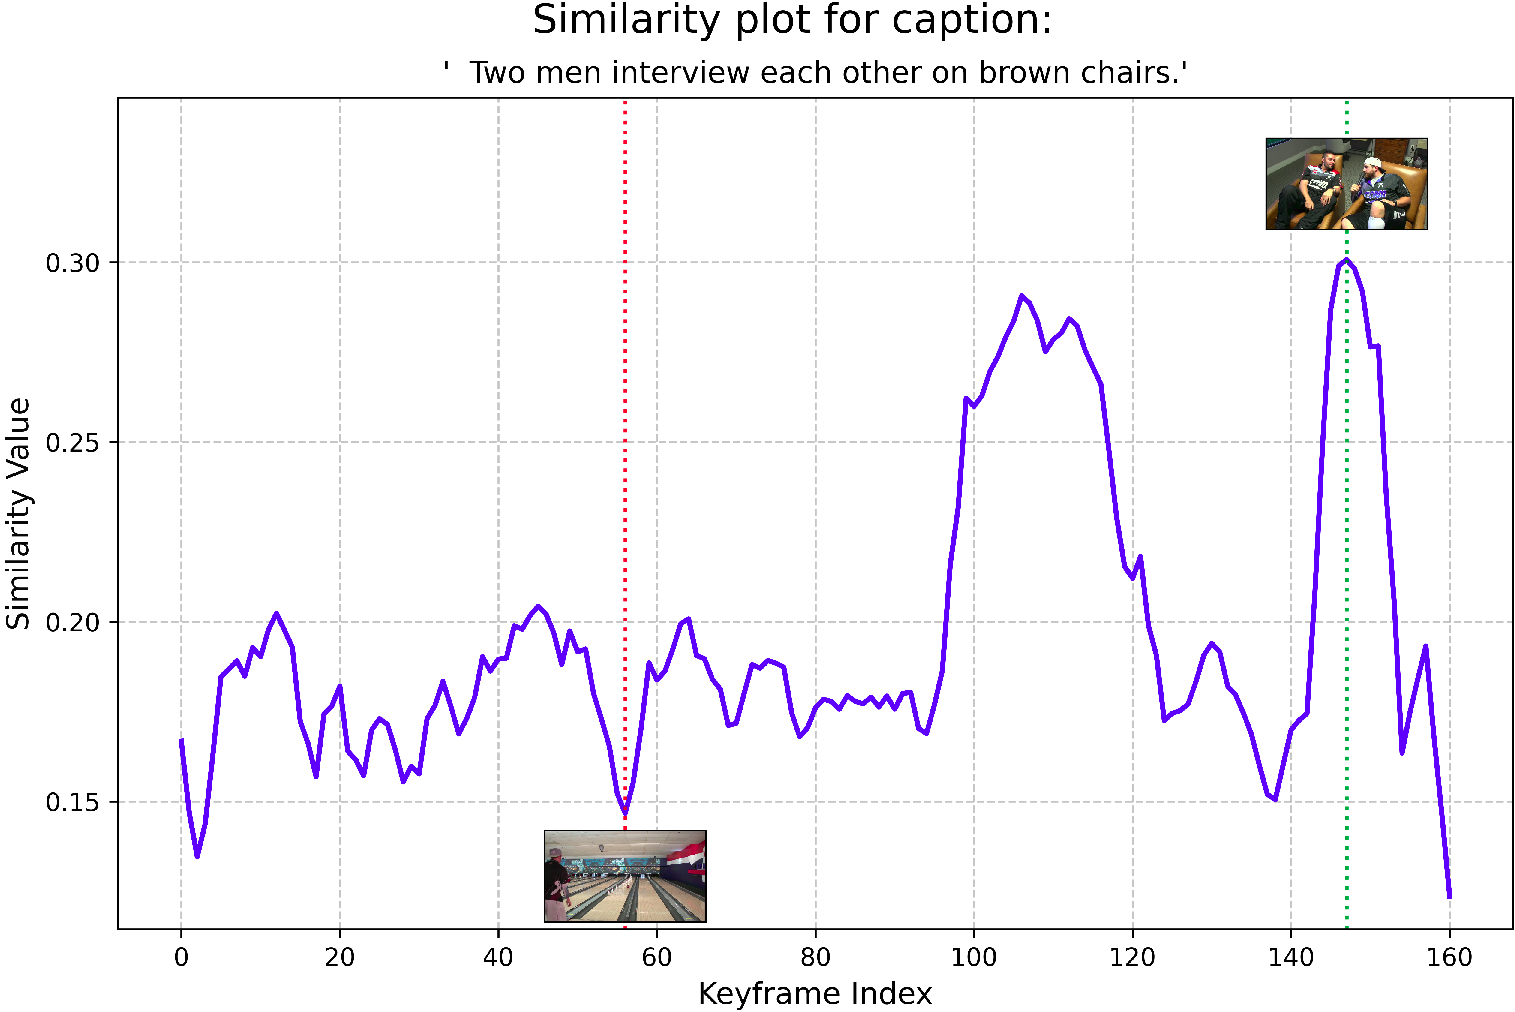
\includegraphics[width=0.9\textwidth, clip=true]{../figures/lang_vis_temp_similarity1.png}
  \caption{Caption-Keyframe similarity score example 1}\label{cap-frame-sim-score-1}
\end{figure}

\begin{figure}[!htb]
  \centering
  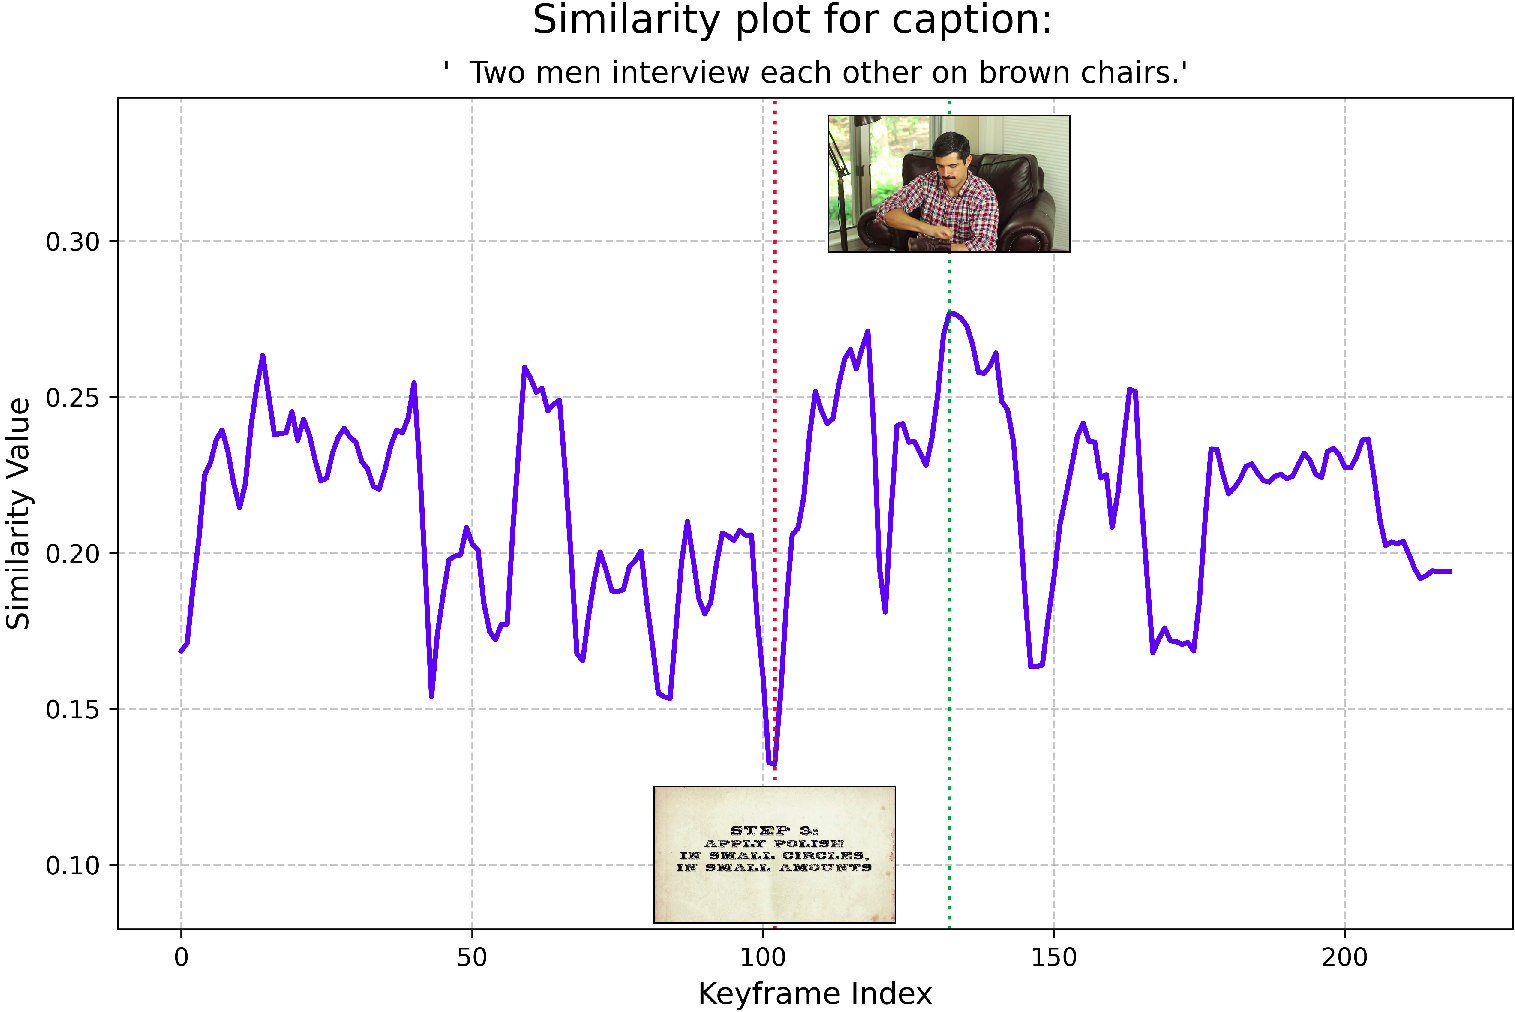
\includegraphics[width=0.9\textwidth, clip=true]{../figures/lang_vis_temp_similarity2.png}
  \caption{Caption-Keyframe similarity score example 2}\label{cap-frame-sim-score-2}
\end{figure}

\clearpage

By taking this same caption and comparing it with another video, we are able to see that, when something that could be vaguely described with it happens, its similarity score increases, as seen in Fig.\ref{cap-frame-sim-score-2}. The other video we used for this comparison is about how to shine shoes - a very different topic from bowling ball trickshots. But when we look at the graph - and particularly at the segment with the highest score - in the keyframe corresponding to that moment we can see something that could be considered as very similar to our caption: a man talking in a black chair. As for the moment with the lowest similarity, it could be anything really, but in our case it was one of the transitions, where the frame shows only text.


\subsubsection{Language-Vision contrastive moments}
Now to give a broader view, we analyze a heatmap of the CLIP embeddings corresponding to every segment's caption of the show shining video and a frame extracted exactly from the middle of it. The results are shown in Fig.\ref{cap-frame-sim-heatmap}. Due to the method we used of extracting the frame in the exact middle and the fact that some segments are very long, whereas the caption refers to a only a short part, the results are exactly perfect, however, a fairly strong match can still be seen along the main diagonal, with much darker colors on the counter-diagonal.

\begin{figure}[!htb]
  \centering
  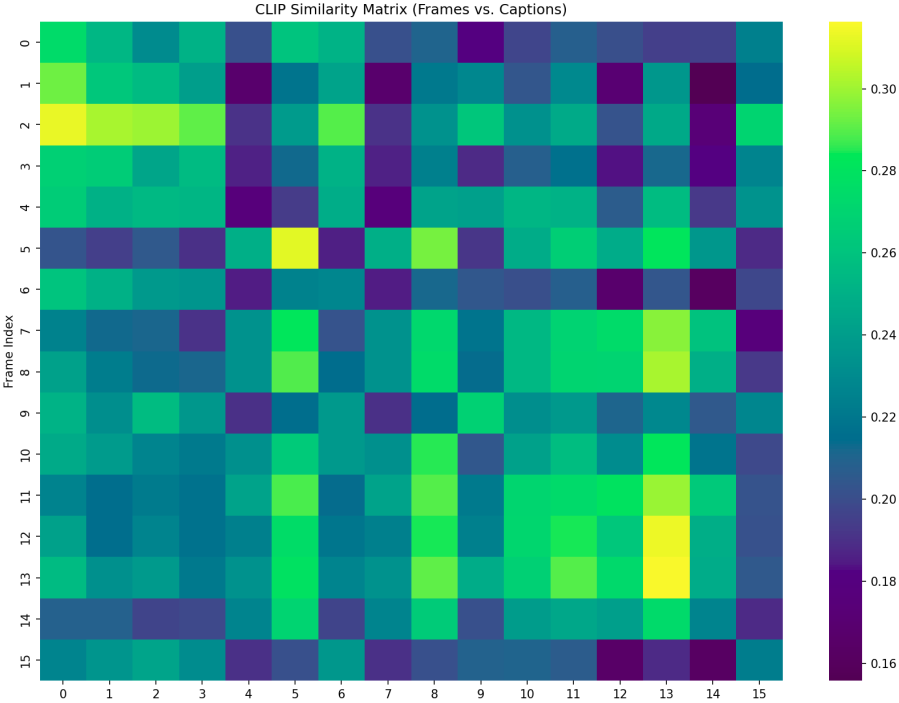
\includegraphics[width=0.9\textwidth, clip=true]{../figures/sim_heatmap.png}
  \caption{Caption-Keyframe similarity heatmap}\label{cap-frame-sim-heatmap}
\end{figure}


Finally, to really visualize the attention that is being given to certain parts of a frame, given a caption, we adapted the provided interpretable visual maps to generate a matrix of visualizations for the same frames and captions used above, seen in Fig.\ref{atent_hm_matrix}. These representations really nail the relationship between what the text describes and what is the image. In particular, if we look at the image resulting of the caption '\textit{The man shines his shoes}' with the corresponding frame for that moment, it is very clear how the attention is being directed at the part of the image where the shoes are, whereas for the same frame, with the caption '\textit{A man is standing inside a bathroom}', the focus shifts upwards - with the hotter areas being the parts of the frame where we can see the man.

\begin{figure}[!htb]
  \centering
  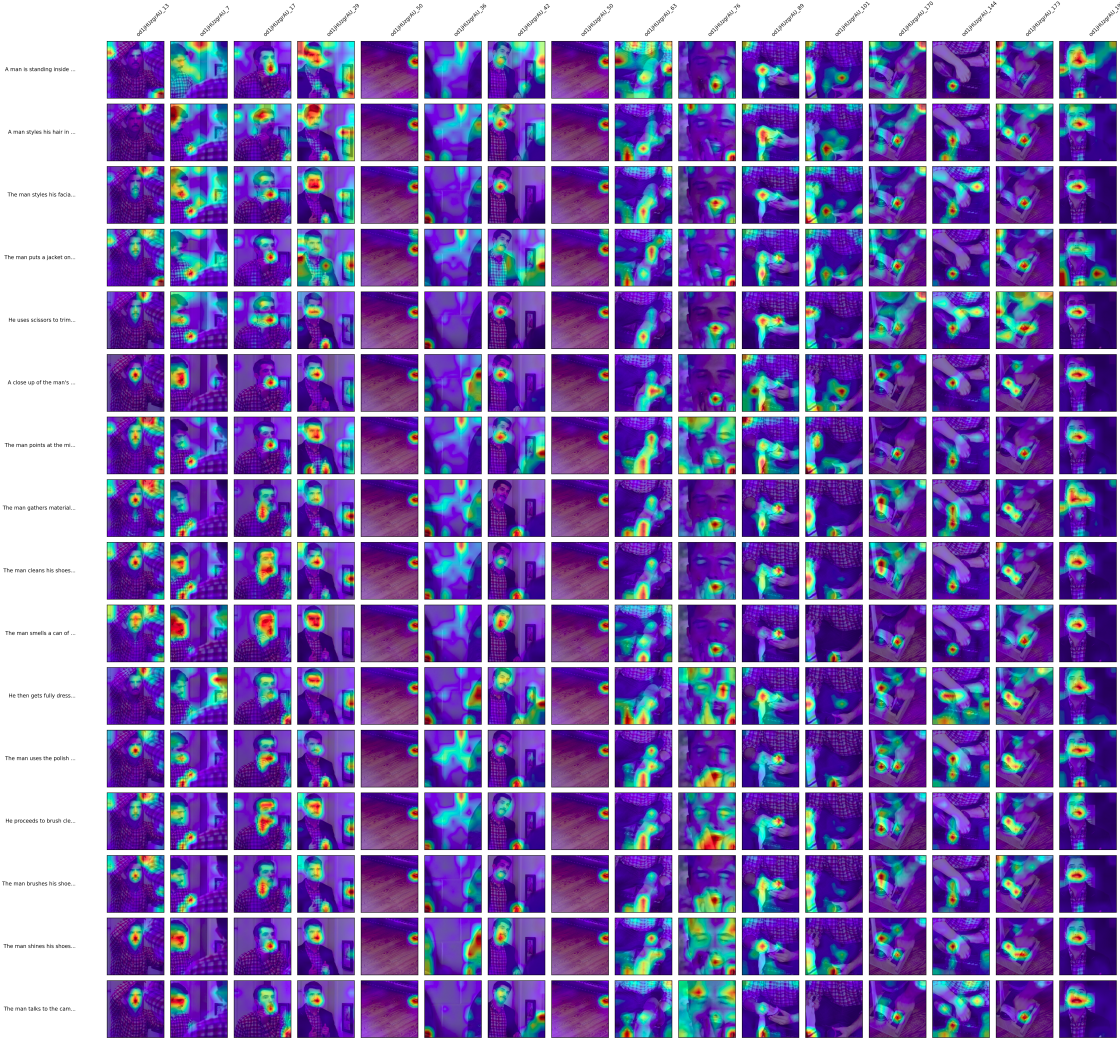
\includegraphics[width=0.9\textwidth, clip=true]{../figures/attention_heatmap_matrix.png}
  \caption{Attention heatmap matrix}\label{atent_hm_matrix}
\end{figure}

\section{Evaluation}

\subsection{Dataset Description}
We used the \href{https://huggingface.co/datasets/HuggingFaceM4/ActivitiyNet_Captions}{ActivityNet Captions dataset}, which provides:

\begin{itemize}
    \item \ensuremath{\sim}20k YouTube videos with natural language descriptions of events,
    \item Timestamp-aligned captions for video moments.
\end{itemize}

In our implementation, we selected from the dataset 10 videos with a reasonable amount of moments. For each:

\begin{itemize}
    \item Keyframes were extracted using PyAV by saving either keyframes or one frame per second.
    \item Corresponding captions were merged and aligned using metadata from three different files: val\_1.json, val\_2.json, and activity\_net.v1-3.min.json.
\end{itemize}

The resulting data was indexed in OpenSearch using custom mappings to support both text-based and embedding-based (knn) search.

\section{Phase 3: Visualizing text with keyframes}

\subsection{Our idea}

When reading a book, say a piece of fiction or romance, as the author paints a picture of the different sceneries and characters, we try to imagine them in our head. As we read, each different word steers our imagination in a slightly different direction, until a full picture is painted. When using a CLIP model to encode a caption, the model is attempting to generate an embedding that is able to encapsulate the meaning and context of that piece of text. Considering this, we could make an analogy between these embeddings and the full picture we paint in our head when reading a book. For this phase, what we attempted was to develop an approach that would allow us to simulate this mechanism, where we picture an image in our mind after every word we read.

\subsection{Our approach}

Simulating this process could be done in many different ways, but with the goal of demonstrating our understanding of the course's topics and technologies, we decided to make the most out of what we had already done and reutilize what we had already implemented within this project. The desired result was a sequence of images that could represent what we imagine in our brain as we read a sequence of text. For obvious reasons we had very moderate expectations of the realism of the result, especially since we were only using the frames of the videos we indexed, but we employed the tools at our disposal to make it as good as possible. %%%%%%%%%% possivelmente melhorar esta ultima parte

\subsubsection{Implemented solution —}

As we have established, what we want is to generate a video (or, more precisely, a sequence of images) given a textual input. For this, we used embeddings generated from that input to query our OpenSearch index for the most similar frames and stitched them all together. Simply using the final generated embedding of our CLIP model for an input would not be enough, as this embedding would not capture the nuance in meaning of each word separately and in sequence. To capture that nuance we would need an embedding for each of our words — or tokens. 
\paragraph{}
In an initial attempt we tried to just split our input in words and encode each of these words separately, but we quickly realized this would not be correct, as the generated embeddings for each word would completely lack any nuance and context of how that word was used. Having concluded this, in the next iteration we decided to pass the input whole and tried to extract the embedding of each token after the final layer, in an attempt to get their contextualized embeddings. When analyzing the result, what we found was that most frames were very similar, if not equal, and did not match in any way the meaning of the word they were representing. It was at this point that we finally got a good grasp of how attention works and how that translates to the embeddings the model computes. By the final layer, the embedding of each token had converged to similar representations of the overall meaning of our input, so we realized this was also not what we wanted. 
\paragraph{}
On the third iteration we finally realized what we needed was the outputted embeddings of the first layer. By this point the model has computed the attention of all of our tokens and updated their embeddings once, resulting in these embeddings being contextualized considering the whole input, but not yet having their individual meanings completely diluted. Using these embeddings, we query our index to get the frame most similar to each token and stitch them together.

\subsubsection{Methods for improving the result —}
By running the previously described solution, what we get is a seemingly nonsensical slideshow of video frames. To simulate a more interesting video, we expanded our implementation to leverage some other tools we had worked with in this project. 
\paragraph{}
Since we had indexed our frames with their ordering number, the first thing we did was use this to get more than one frame per token. To be precise, we fetched the next and previous frame, if they existed, of the most similar frame. Since one of these frames could be from a separate section of the video, applying this blindly could be useless, or even worsen the video. To mitigate this, we also calculate the similarity between the main frame — the one we get from querying OpenSearch with a token's embedding — and the previous and next frames. If their similarities are lower than a threshold we defined, we discard them. 
\paragraph{}
This technique allowed for less jumping around but, from one word to the next, the frames are still generally very different, resulting in very noticeable transitions. With this in mind, we used something that had not yet been explored in the context of this project: a video interpolation model. After some research on available models, we settled on RIFE (Real-Time Intermediate Flow Estimation), which is able to generate intermediate frames given two distinct images. Each token in our input translates to a scene of 1 to 3 frames in the generated video, so, by feeding the last frame corresponding to a token and the first frame corresponding to the next token to this generative model, we get a much smoother transition between scenes. It's worth noting that the model we used is fairly small, so it was not capable of generating particularly detailed or high quality images, but we considered this a feature, not a bug, since it resulted in the dream-like effect we were aiming for since the beginning.
\paragraph{}
The approach we adopted involved identifying whether two consecutive frames (i.e., the last frame of a token and the first of the next token) represented different scenes. If they did, we considered that a transition point and used RIFE to generate a configurable number of interpolated frames between them. We developed a pipeline that processed the sequence of selected frames, detecting transitions, and running the model only when necessary to avoid generating intermediate frames between already adjacent frames from the same shot.
\paragraph{}
Although we felt that transitions needed this interpolation step the most, we wondered what the result would be if we interpolated every two consecutive frames, including adjacent frames, considering that even the adjacent frames we had indexed had a small gap between them. The result was better than the previous version, in which only frames corresponding to transitions would be interpolated. After some experimentation, we found that with minor changes in our implementation we could easily alternate between the two options.
\paragraph{}
One challenge we encountered was that RIFE sometimes produced duplicate or near-identical frames at the end of its output sequence, which could create unnatural pauses or stutters in the final video. To mitigate this, we implemented a frame comparison mechanism to detect and remove redundant images from the output. We also ensured that every interpolated sequence maintained consistent naming and ordering so that the final video could be stitched together seamlessly.
\paragraph{}
The final result was a more continuous video that reflected the evolving context of the input text. Although the video still exhibits some degree of abstraction and randomness due to the limitations of using unrelated indexed video frames, the incorporation of RIFE allowed us to convey a sense of narrative and imagination, which is precisely what we set out to simulate.

\end{document}
